
%(BEGIN_QUESTION)
% Copyright 2006, Tony R. Kuphaldt, released under the Creative Commons Attribution License (v 1.0)
% This means you may do almost anything with this work of mine, so long as you give me proper credit

Steam drum water level measurement is actually a form of interface level measurement, because high-pressure steam is significantly denser than air under ambient conditions:

$$\includegraphics[width=15.5cm]{i00316x01.eps}$$

Making this situation even more complex is the fact that the densities of both the water and the steam change as boiler pressure and temperature change.  Identify what happens to water density and steam density as both pressure and temperature increase, and explain why.

\underbar{file i00316}
%(END_QUESTION)





%(BEGIN_ANSWER)

As boiler temperature increases, the water density decreases.  For saturated steam conditions (i.e. water and steam in direct contact with each other in the same vessel), pressure and temperature are directly related.  So, as temperature in the steam drum increases, pressure must also.  This increase in pressure causes the steam to become denser as the steam molecules become packed closer together.

\vskip 10pt

Just to give you an example of how significant these density changes are at high pressure (e.g. power generation boilers), consider the following values:

\begin{itemize}
\item{} Boiling (saturated) water density at 2,425 PSIG = 35.49 lb/ft$^{3}$
\item{} Saturated steam density at 2,425 PSIG = 7.33 lb/ft$^{3}$
\end{itemize}

%(END_ANSWER)





%(BEGIN_NOTES)


The data for steam and water given in the answer was taken from Rosemount's Application Data Sheet \#00800-0100-3055.

%INDEX% Measurement, level: steam drum (vapor density compensation)
%INDEX% Process: boiler steam drum water level

%(END_NOTES)


